

\subsection{Terrein}
Het terrein kan in wezen allerlei vormen hebben, voorwaarde hierbij is dat het een eerlijk terrein is voor beide teams. Een team mag dus geen voordeel hebben dankzij de kaart. Een mogelijke manier om dit te bereiken is door de kaart symmetrisch te maken. We eisen bovendien dat de kaart rechthoekig is. 

Op het terrein zijn twee commandocentra geplaatst, voor beide teams een commandocentrum. Het kan gewenst zijn dat elk team bij de start van het spel ook al een aantal extra torens heeft ter bescherming van het commandocentrum. Over het terrein zijn een aantal delfplaatsen verdeeld. Deze zijn eerlijk verdeeld over de kaart. Andere obstakels mogen aanwezig zijn, maar zijn niet noodzakelijkerwijs aanwezig. In figuur \ref{fig:map1} en \ref{fig:map2} zijn twee mogelijke beginconfiguraties van het spel getoond.
\begin{figure}[h]
\begin{subfigure}{0.5\textwidth}
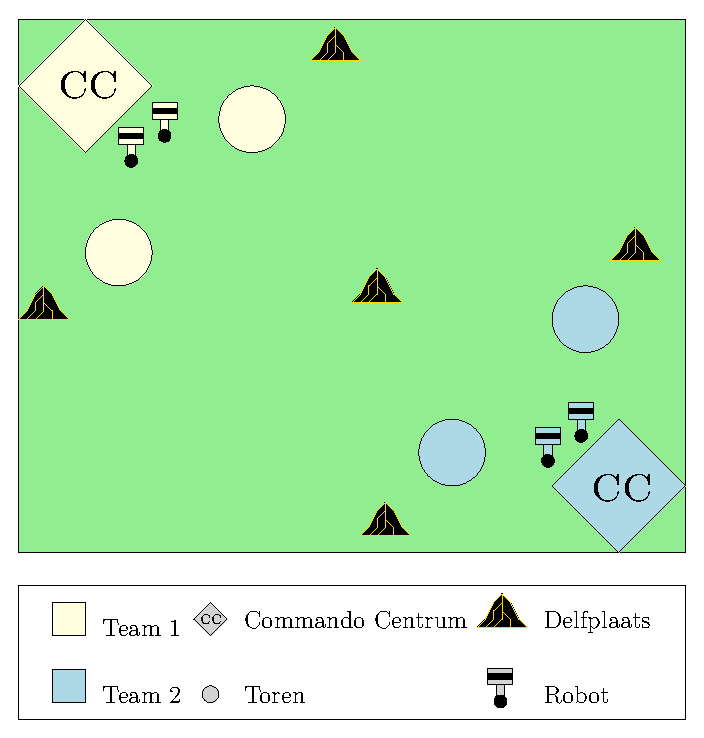
\includegraphics[width=\textwidth]{Graphics/Map1.eps}
\caption{Een bijna vierkant terrein met vier spelers}
\label{fig:map1}
\end{subfigure}\hspace{10mm}
\begin{subfigure}{0.5\textwidth}
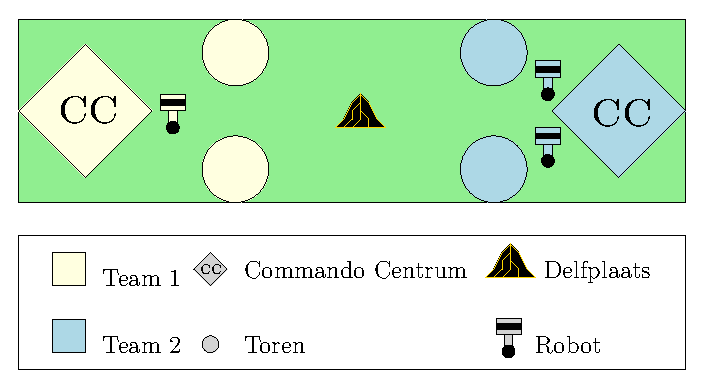
\includegraphics[width=\textwidth]{Graphics/Map2.eps}
\caption{Een breed terrein met drie spelers}
\label{fig:map2}
\end{subfigure}
\caption{Twee verschillende beginconfiguraties van het spel}
\end{figure}
\subsection{Spelers}
Een speler behoort tot een van beide teams, spelers van een bepaald team zijn te identificeren door kleuren. De speler ziet de wereld vanuit de positie van zijn robot. Hij kan de kijkrichting aanpassen, zodat deze in elke willekeurige richting kan staan.  De speler heeft een lasergeweer waarmee hij op andere spelers en torens kan schieten om deze te vernietigen. Als een speler schiet, dan wordt geschoten in de huidige kijkrichting van de robot. Bij het begin van het spel heeft de robot nog een volledig harnas. Zodra de speler wordt geraakt, wordt de conditie van het harnas slechter. Het is echter niet mogelijk dat een speler het harnas van een andere speler uit hetzelfde team beschadigt.
\FloatBarrier
Een speler gaat dood als zijn harnas kapot is. In dat geval zal hij na een bepaalde hoeveelheid tijd terugkeren bij het commandocentrum met een volledig harnas. De conditie van het harnas kan op geen enkele andere dan de hierboven beschreven manieren veranderen. Ook kan een speler gebouwen bouwen, hiervoor gebruikt hij goud uit de kas van het team. De spelers kunnen op het grondvlak bewegen met een vaste snelheid in elke richting. De enige voorwaarde hierbij is dat de spelers op de kaart blijven en niet door een gebouw lopen. Het is dus wel mogelijk dat spelers door elkaar heen kunnen lopen. De spelers besturen hun karakter in een zogenaamde \emph{third person view}.


\FloatBarrier
\subsection{Gebouwen}
Er zijn drie soorten gebouwen: torens (gebouwen die op spelers en andere gebouwen in hun bereik kunnen schieten), mijnen (gebouwen die over een delfplaats kunnen worden gebouwd om de inkomsten van het team te vergroten) en een commandocentrum (het belangrijkste gebouw voor het team, als dit gebouw kapot is, heeft het bijbehorende team verloren). Alle gebouwen behoren tot een van beide teams, deze gebouwen kunnen weer ge\"identificeerd worden door de kleur van het gebouw.

\subsection{Verzamelbare voorwerpen}
Er is maar \'e\'en verzamelbaar voorwerp: een muntje. Een muntje wordt achtergelaten door spelers die dood gaan en torens die worden vernietigd. Een muntje heeft een bepaalde waarde in goud. De waarde van het muntje is proportioneel aan de gezamenlijke kas van het team waarvan de speler is doodgegaan. Als een toren is vernietigd, dan is de waarde van het muntje proportioneel aan de kosten van de toren. De waarde van het muntje moet echter altijd kleiner zijn dan de kosten van de toren. Gedurende een spel moeten deze proporties vast zijn.

Als een speler doodgaat, wordt bovendien nog de waarde van het muntje afgetrokken van de gezamenlijke kas van die speler. Een muntje kan vervolgens opgepakt worden door alle spelers. Het muntje is dus het voedsel element in ons spel. De waarde van het muntje zal dan toegevoegd worden aan de kas van het bijbehorende team.

\subsection{Initialisatie}
Bij de start van het spel staan alle spelers bij het commandocentrum. Zoals al eerder gezegd, hebben alle spelers dan nog een volledig harnas. Bovendien heeft elk team een zekere positieve hoeveelheid goud in de gezamenlijke kas, die voor beide teams natuurlijk gelijk moet zijn. Er kunnen minstens twee mijnen gebouwd worden met deze hoeveelheid goud.

\section{Optioneel}
We hebben ook een aantal plannen voor uitbreiding van het spel, vooral om het uitgebreider te maken en leuker om te spelen. De volgende idee\"en staan op ons lijstje, waarbij de idee\"en gesorteerd zijn op aflopende volgorde van belangrijkheid.
\begin{itemize}
  \item Extra goud, de gezamenlijke kas wordt periodiek met een vaste hoeveelheid verhoogd. Dit is dan additief met eventuele mijnen. Wij verwachten dat dit weinig tijd kost.
  \item Oorlogsmist, de robots hebben een beperkt zichtveld. Dit voorkomt dat spelers vanaf hun commandocentrum alle activiteiten van de tegenstanders kunnen zien. Wij denken dat dit weinig tijd kost.
  \item Plattegrond, zodat spelers een globaal overzicht krijgen van wat er op de kaart gebeurt. Dit kan eventueel ook weer met een oorlogsmist zijn, zodat de spelers alleen een gedeelte van het plattegrond kunnen zien, waar teamgenoten in de buurt staan. Wij vermoeden dat dit niet veel tijd kost.
  \item Muren, als een extra type gebouw. Onze bedoeling hierbij is dat deze muren relatief goedkoop zijn om te bouwen. Dit geeft een team meer opties om hun commandocentrum of delfplaatsen te beschermen. Bovendien geeft het de extra mogelijkheid om een veilige plek te cre\"eren, waarvandaan tegenstanders aangevallen kunnen worden. Wij voorzien dat dit een kleine hoeveelheid tijd kost. 
  \item Ontwikkelingen, de spelers krijgen ontwikkelingspunten tijdens het spel. Deze kunnen worden verdiend door het uitschakelen van spelers, werkers, infanterie en het vernietigen van gebouwen. Hiermee kunnen de spelers bijvoorbeeld de eigenschappen van hun robot verbeteren, zoals de snelheid van lopen en hoe sterk het harnas is. Ook is het mogelijk om sterkere wapens te kopen. Wij denken dat dit veel tijd kost, aangezien een `winkel' gemaakt moet worden waar deze punten gespendeerd kunnen worden. Ook moeten de eigenschappen van een speler dynamisch gemaakt worden.
  \item Werkers, dit zijn computergestuurde robots. Zodra een speler daartoe opdracht geeft, komen werkers uit het commandocentrum van het bijbehorende team om een gebouw neer te zetten. Dit vervangt de oude mogelijkheid van spelers om te bouwen. Een gevolg van deze aanpassing is dat het langer duurt om een gebouw te bouwen als de afstand van de bouwplaats tot het commandocentrum groter is. Bovendien wordt het mogelijk om het bouwen van het andere team te vertragen door de werkers uit te schakelen. Dit kost heel veel tijd, aangezien de werkers gedistribueerd bestuurd worden. Hiervoor is dus een soort gedistribueerde kunstmatige intelligentie nodig. Dit is een uitdaging. Merk ook op, dat deze computergestuurde robots niet door de gebouwen horen te lopen, waardoor deze kunstmatige intelligentie totaal niet triviaal is.
  \item Infanterie, ook dit zijn computergestuurde robots. Deze kunnen door spelers worden gekocht, vanaf het commandocentrum lopen ze naar gebouwen van het andere team om deze gebouwen aan te vallen. Dit kost nog meer tijd dan de werkers, aangezien de infanterie niet tussen twee vaste punten zich moeten verplaatsen, maar ook gebouwen moeten kunnen aanvallen. 
\end{itemize} 